\documentclass[mathserif,18pt,xcolor=table]{beamer}
\usepackage{amsmath}
\usepackage{amssymb}
\usepackage{bbm}
\usepackage{ulem}
\usepackage{feynmp-auto}
%\usepackage{slashed}
\usepackage[absolute,overlay]{textpos}
\usepackage{graphicx}
\usepackage{listings}
\usepackage{epsfig}
\usepackage{hyperref}
\usepackage{tikz}
\usetikzlibrary{calc}
\usepackage{enumerate}
%\usepackage{fixltx2e} % buggy
\usepackage[compatibility=false]{caption}
\usepackage{subcaption} % doesn't work with subfigure
%\usepackage{pdfpages}
\usepackage{setspace}
\usepackage{verbatim}

%\usepackage{siunitx}

\DeclareRobustCommand{\orderof}{\ensuremath{\mathcal{O}}}

\definecolor{dukeblue}{RGB}{0,0,156}
\definecolor{dukedarkblue}{RGB}{0,26,87}
\definecolor{dukeblack}{RGB}{79,79,79}
\definecolor{dukegray}{RGB}{79,79,79}
\definecolor{dukesecbrown}{RGB}{217,200,158}
\definecolor{dukesecblue}{RGB}{127,169,174}
\mode<presentation> {
  \usetheme{Boadilla}  
  \setbeamercovered{invisible}
  \setbeamertemplate{navigation symbols}{}  
  \setbeamertemplate{frametitle}[default][center]
  \setbeamertemplate{bibliography item}{\insertbiblabel}
  \setbeamerfont{frametitle}{series=\bfseries,parent=structure}
  \setbeamerfont{subtitle}{size=\scriptsize,series=\bfseries,parent=structure}
  \setbeamerfont{author}{size=\scriptsize,parent=structure}
  \setbeamerfont{institute}{size=\small,series=\bfseries,parent=structure}
  \setbeamerfont{date}{size=\scriptsize,parent=structure}
  \setbeamerfont{footline}{size=\tiny,parent=structure}
  \setbeamercolor{normal text}{bg=white,fg=dukeblack}
  \setbeamercolor{structure}{fg=dukeblue}
  \setbeamercolor{alerted text}{fg=red!85!black}
  \setbeamercolor{item projected}{use=item,fg=black,bg=item.fg!35}
  \setbeamercolor*{palette primary}{use=structure,fg=white, bg=dukeblue}
  \setbeamercolor*{palette secondary}{use=structure,bg=dukedarkblue,fg=white}
  \setbeamercolor*{framesubtitle}{fg=dukegray}
  \setbeamercolor*{block title}{parent=structure,fg=black,bg=dukeblue}
  \setbeamercolor*{block body}{fg=black,bg=dukeblack!10}
  \setbeamercolor*{block title alerted}{parent=alerted text,bg=black!15}
  \setbeamercolor*{block title example}{parent=example text,bg=black!15}
}

\makeatletter
\setbeamertemplate{footline}{
  \leavevmode
  \hbox{%
    \begin{beamercolorbox}[wd=.333333\paperwidth,ht=2.25ex,dp=1ex,center]{author in head/foot}%
      \usebeamerfont{author in head/foot}\insertshortauthor%
    \end{beamercolorbox}%
    \begin{beamercolorbox}[wd=.333333\paperwidth,ht=2.25ex,dp=1ex,center]{title in head/foot}%
      \usebeamerfont{title in head/foot}\insertshorttitle%
    \end{beamercolorbox}%
    \begin{beamercolorbox}[wd=.333333\paperwidth,ht=2.25ex,dp=1ex,right]{date in head/foot}%
      \usebeamerfont{date in head/foot}\insertshortdate{}\hspace*{2em}%
      \insertframenumber{} / \inserttotalframenumber\hspace*{2ex}%
%      \insertframenumber{} / 11\hspace*{2ex}% TODO hard code to page number before backup!!
    \end{beamercolorbox}}%
  \vskip0pt%
}
\makeatother


\AtBeginSection{\frame{\sectionpage}}


\defbeamertemplate{section page}{mine}[1][]{%
  \begin{centering}
    {\usebeamerfont{section name}\usebeamercolor[fg]{section name}#1}
    \vskip1em\par
    \begin{beamercolorbox}[sep=12pt,center]{part title}
      \usebeamerfont{section title}\insertsection\par
    \end{beamercolorbox}
  \end{centering}
}


\usepackage[protrusion=true,expansion=true]{microtype}
\usepackage{amsmath}
\renewcommand*{\thefootnote}{\fnsymbol{footnote}}
\title[Group Project 1]{Group Project 1\newline Random Walk, Diffusion and Cluster Growth}
\author[Xu, Epland, Li, Cohen]{{\small Yuanyuan Xu, Matthew Epland, Xiaqing Li, Wesley Cohen}}
\institute{Duke University}
%\date{\today}
\date{March 25, 2016}
\hypersetup{
    breaklinks,
    baseurl       = http://,
    pdfborder     = 0 0 0,
    pdfpagemode   = UseNone,% do not show thumbnails or bookmarks on opening
    pdfstartpage  = 1,
    bookmarksopen = true,
    bookmarksdepth= 2,% to show sections and subsections
    pdfauthor     = {\@author},
    pdftitle      = {\@title},
    pdfsubject    = {},
    pdfkeywords   = {}}

\titlegraphic{
\includegraphics[height=2cm]{logos/duke_logo.pdf}}

% Point to nice top level directory
\graphicspath{{../output/plots_for_paper/}}

\begin{document}

\beamertemplateballitem
\frame{\titlepage}
\addtobeamertemplate{frametitle}{}{}


\begin{frame}
  \frametitle{Introduction}
  \begin{itemize}
    \item Bullet point text here TODO
  \end{itemize}

\end{frame}

\begin{frame}
  \frametitle{DLA Cluster: RNG Seed $= 6$}
\begin{figure}
  \centering
  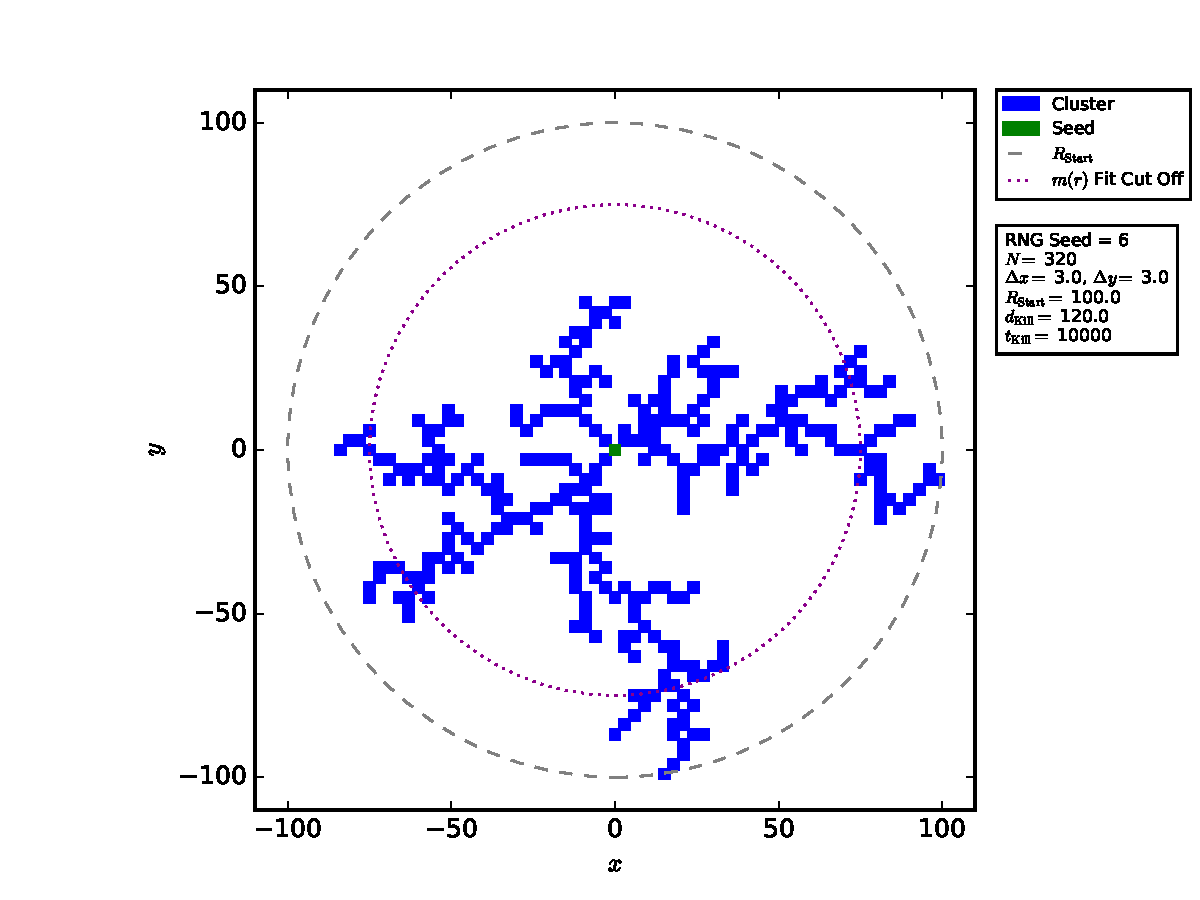
\includegraphics[width=0.9\textwidth]{problem_3/large_cluster_seed_num_6.pdf}
\end{figure}
\end{frame}

\begin{frame}
  \frametitle{DLA Cluster Mass: RNG Seed $= 6$}
\begin{figure}
  \centering
  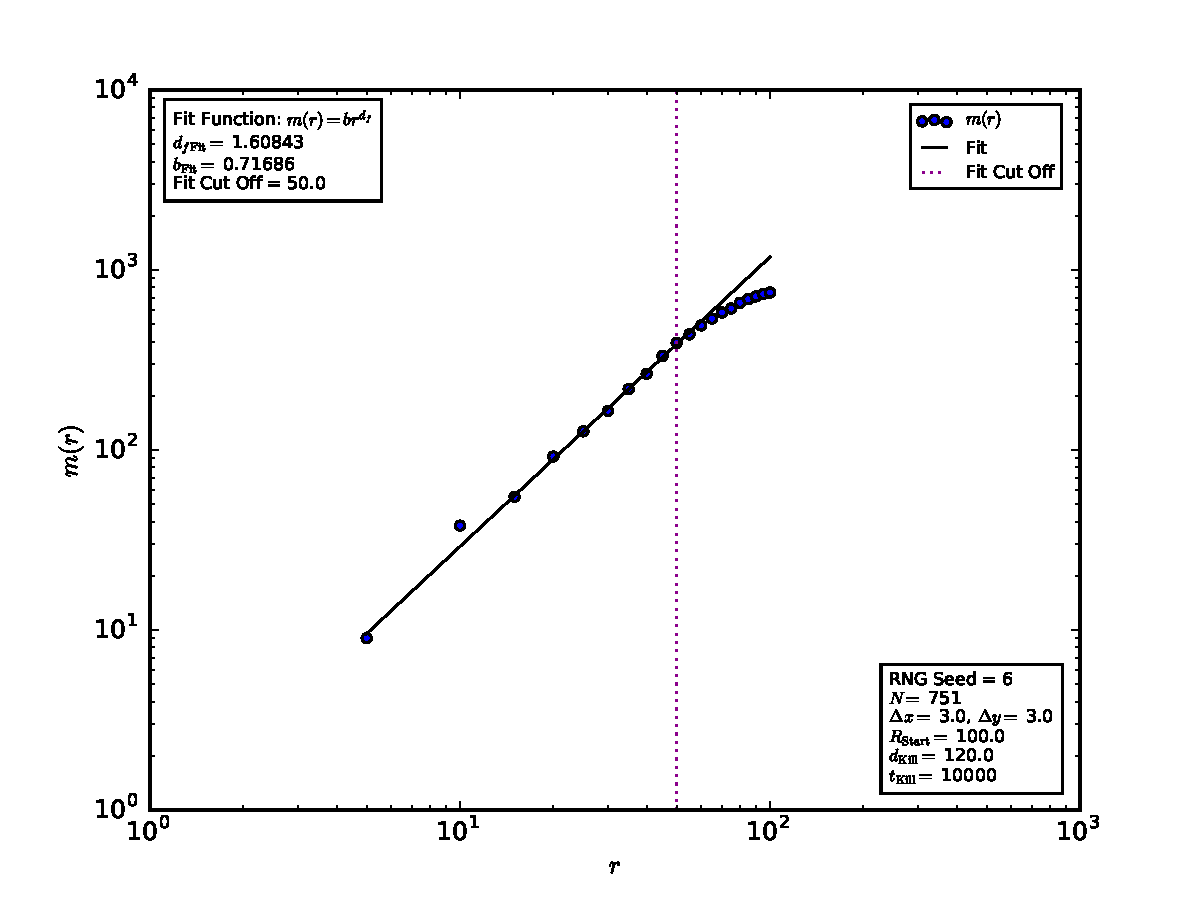
\includegraphics[width=0.9\textwidth]{problem_3/large_cluster_mass_seed_num_6.pdf}
\end{figure}
\end{frame}

\begin{frame}
  \frametitle{DLA Cluster: RNG Seed $= 10$}
\begin{figure}
  \centering
  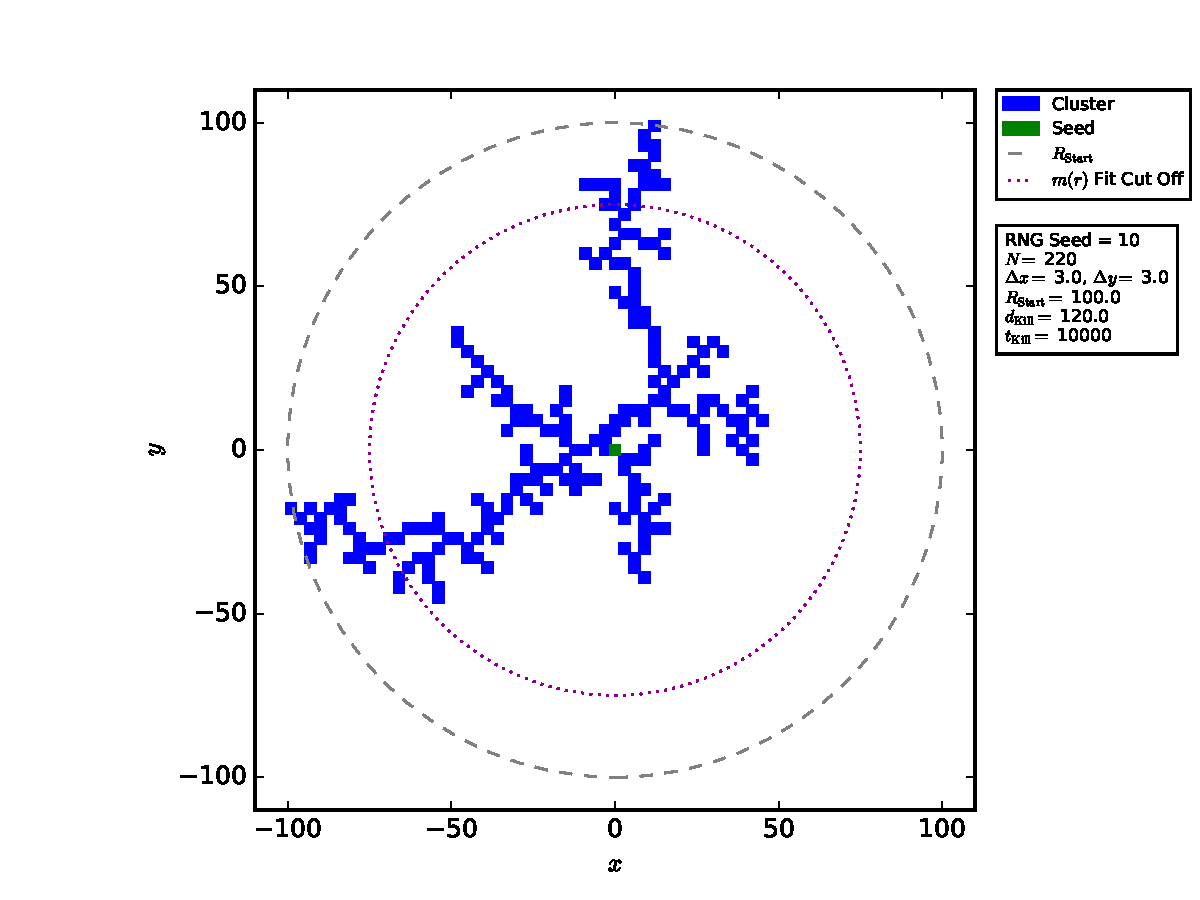
\includegraphics[width=0.9\textwidth]{problem_3/large_cluster_seed_num_10.pdf}
\end{figure}
\end{frame}

\begin{frame}
  \frametitle{DLA Cluster Mass: RNG Seed $= 10$}
\begin{figure}
  \centering
  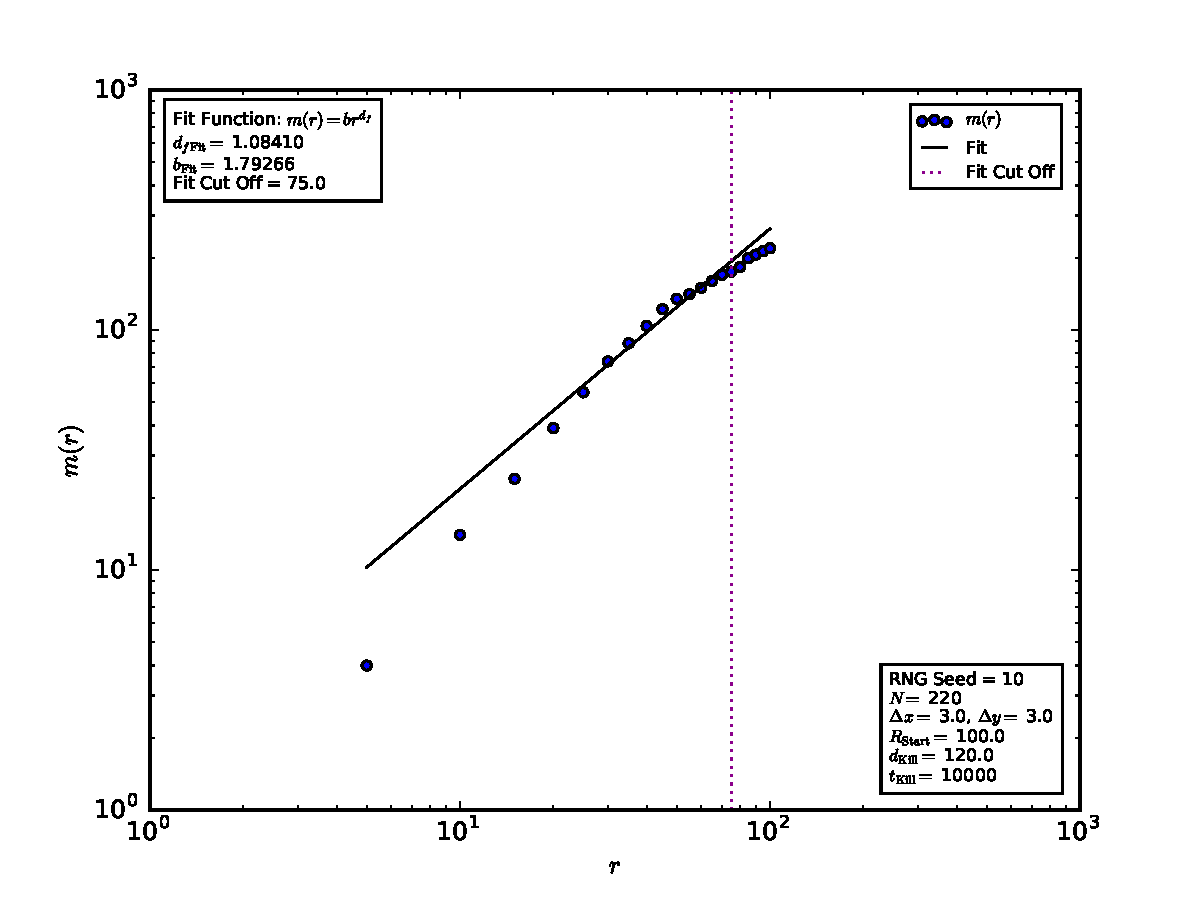
\includegraphics[width=0.9\textwidth]{problem_3/large_cluster_mass_seed_num_10.pdf}
\end{figure}
\end{frame}

\begin{frame}
  \frametitle{DLA Cluster: RNG Seed $= 12$}
\begin{figure}
  \centering
  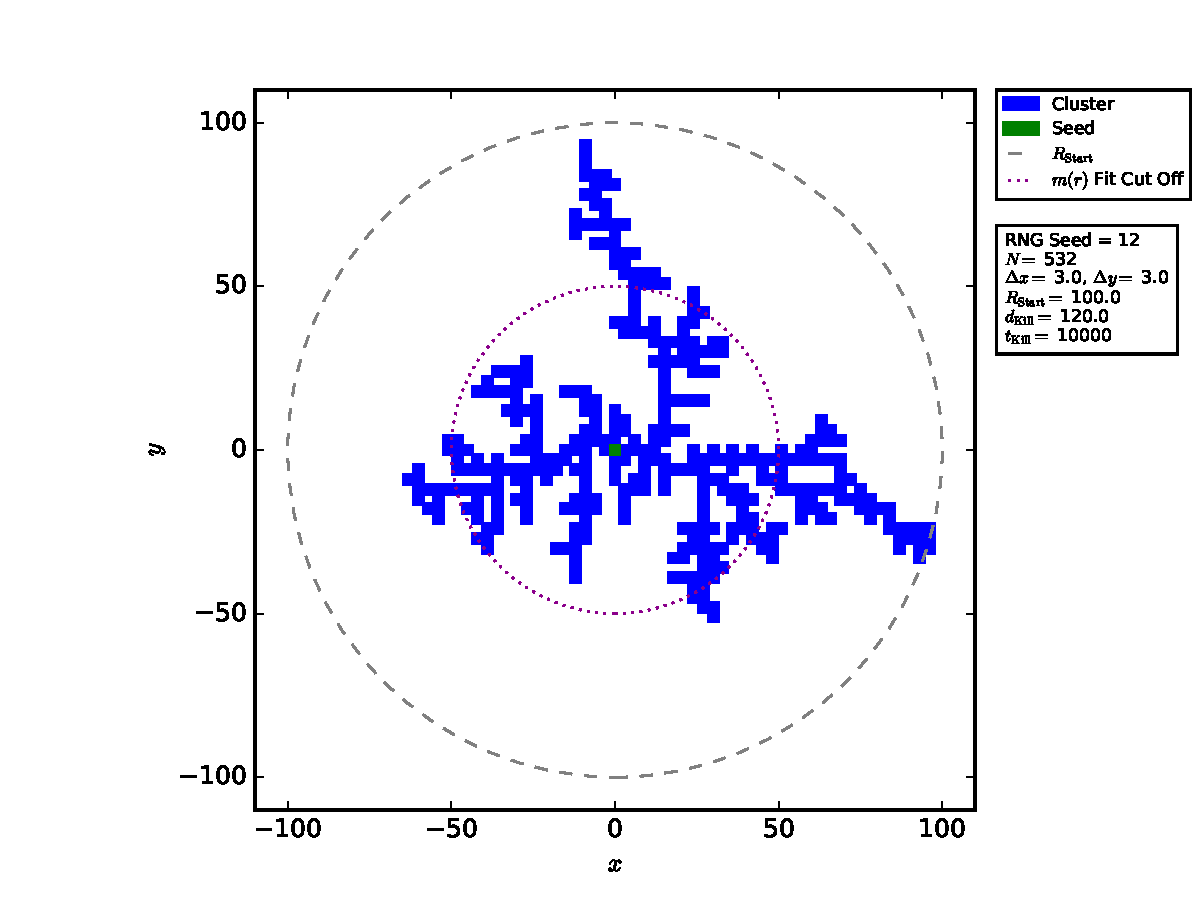
\includegraphics[width=0.9\textwidth]{problem_3/large_cluster_seed_num_12.pdf}
\end{figure}
\end{frame}

\begin{frame}
  \frametitle{DLA Cluster Mass: RNG Seed $= 12$}
\begin{figure}
  \centering
  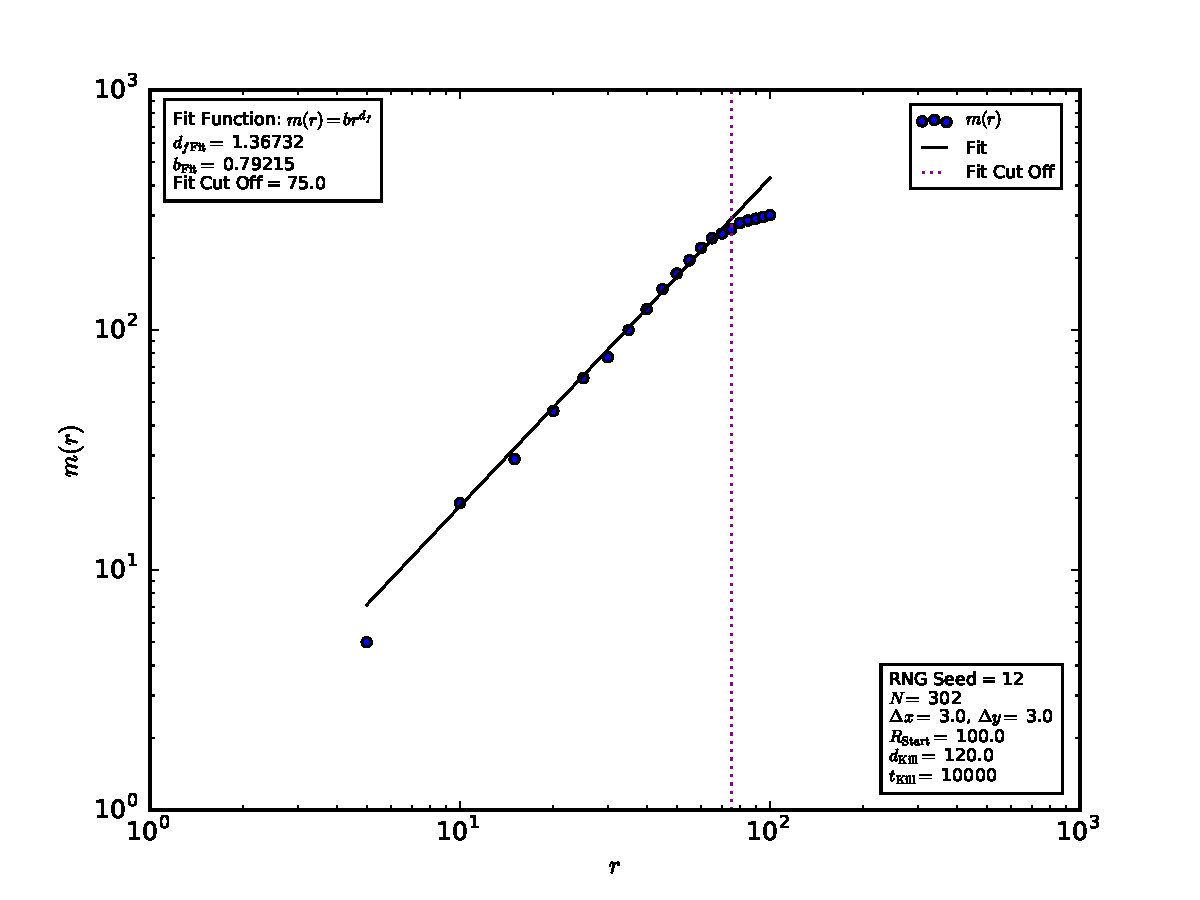
\includegraphics[width=0.9\textwidth]{problem_3/large_cluster_mass_seed_num_12.pdf}
\end{figure}
\end{frame}

\begin{frame}
  \frametitle{Fractal Dimensionality}

  \begin{itemize}
    \item Running over 10 different RNG seeds we find:
    \begin{itemize}
      \item $\left<d_{f}\right> = 1.30$, with Std. Dev. $= 0.10$ 
    \end{itemize}
  \end{itemize}

% You can position text/figures/anyting at an arbitrary position with textblock*
\begin{textblock*}{0.9\textwidth}(1.4cm,8.5cm) % {block width} (coords) note coords are from upper left corner
{\tiny All $d_{f\,\mathrm{fit}} = 1.3347,\,1.3463,\,1.4241,\,1.3854,\,1.0841,\,1.3420,\,1.3673,\,1.2641,\,1.2410,\,1.1970$}
\end{textblock*}

\end{frame}




\end{document}

%%%%%%%%%%%%%%%%%%%%%%%%%%%%%%%%%%%%%%%%%%%%%%%%%%%%%%%%%%%%%%%%%%%%

% Backup
\begin{frame}
    \begin{center}
    \usebeamerfont{frametitle}Backup
    \end{center}
\end{frame}

% bib
\begin{frame}%[allowframebreaks]
        \frametitle{References}
	\bibliographystyle{../bib_files/atlasBibStyleWoTitle}
{\scriptsize
        \bibliography{../bib_files/my_bib.bib}
}
\end{frame}


